\documentclass{article}
\usepackage{nips07submit_e,times}
\usepackage{graphicx}
\usepackage{amssymb}
\usepackage{amsmath}
\usepackage{amsfonts}
\usepackage{multirow}
%\renewcommand{\familydefault}{\sfdefault}
%\documentclass{llncs}
%
%\pagestyle{headings}
%\usepackage{amsmath}
\newcommand{\new}{\newcommand}
\new{\bg}{\begin}
\new{\lp}{\left(}
\new{\rp}{\right)}


\newcommand{\xx}{\mathcal{X}}
\newcommand{\yy}{\mathcal{Y}}
\newcommand{\rr}{\mathbb{R}}

\new{\iii}{\begin{enumerate}}
\new{\fff}{\end{enumerate}}
\new{\iiii}{\begin{itemize}}
\new{\ffff}{\end{itemize}}
\new{\mfi}{\begin{eqnarray*}}
\new{\mff}{\end{eqnarray*}}
\new{\mfni}{\begin{eqnarray}}
\new{\mfnf}{\end{eqnarray}}
\new{\beeq}[2]{\begin{equation}\label{#1}{#2}\end{equation}}
\new{\eqn}[1]{~(\ref{#1})}

\new{\room}{\ \ \ \ }
\new{\card}{\#}


\new{\nor}[1]{\|{#1}\|}
\new{\normi}[1]{\left\|{#1}\right\|_{\infty}}
\new{\scal}[2]{\left\langle{#1},{#2}\right\rangle}
\new{\scalh}[2]{\left\langle{#1},{#2}\right\rangle_\hh}
\new{\set}[1]{\{{#1}\}}
% GENERAL MACRO
%%%%%%%%%%%%%%%%%%%%%%%%%%%%
%\new{\rone}{{\mathrm{I\hskip-2.2pt R}}}
\new{\com}{{\mathbb C}}
\new{\rone}{{\mathbb R}} 
\new{\nat}{{\mathbb N}}

\new{\fz}{f_\vz}
\new{\fzlo}{\overline{f}_\vz^\la}
\new{\rd}{\rone^\dm}
\new{\ed}{{\mathbb E}}
%\new{\nat}{{\mathrm{I\hskip-2.2pt N}}}
%\new{\com}{{\mathrm{I\hskip-2.2pt C}}}

%
%\new{\rd}{{\mathrm{I\hskip-2.2pt R}}^\dm}
%\new{\ed}{{\mathrm{I\hskip-2.2pt E}}^\dm}
\new{\argmin}{\operatornamewithlimits{argmin}}
\new{\argmax}{\operatornamewithlimits{argmax}}
\new{\Prob}[1]{\mathrm{P}\left[\, #1 \right]}
\new{\E}{{\mathbb E}}
\new{\eps}{\varepsilon}
%\new{\nor}[1]{\left\|{#1}\right\|}
%\new{\scal}[2]{\left\langle{#1},{#2}\right\rangle}

%LEARNING MACRO
%%%%%%%%%%%%%%%%%%%%%%%%%%%%%
\new{\marg}{\rho_X}
\new{\prob}{\rho}
\new{\dm}{d}
\new{\tr}{\vz}
\new{\n}{n}
\new{\vb}{{\mathbf b}}
\new{\vf}{{\mathbf f}}
\new{\vl}{\bar{\ell}}
\new{\vx}{{\mathbf x}}
\new{\vy}{{\mathbf y}}
\new{\vz}{{\mathbf z}}
\new{\vc}{{\mathbf c}}
\new{\vu}{{\mathbf u}}
\new{\vv}{{\mathbf v}}
%\new{\k}{{\mathcal k}}
%\new{\kx}{{\mathcal k}_x}
\new{\kk}{K}
\new{\s}{K^s}
\new{\kkx}{K_x}
\new{\w}{W}
\new{\wx}{\w_x}
\new{\WW}{{\mathbf W}}
\new{\DD}{{\mathbf D}}
\new{\LL}{{\mathbf L}}
\new{\LS}{{\mathbf L}_{s}}
\new{\LR}{{\mathbf L}_{r}}
\new{\II}{{\mathbf I}}
\new{\KK}{{\mathbf K}}
\new{\ka}{\kappa}
\new{\ls}{\ell}
\new{\err}{{\mathcal E}}
\new{\emp}{{\mathcal E}_z}
\new{\hh}{{\mathcal H}}
\new{\oo}{{\mathcal G}}
\new{\ff}{{\mathcal F}}
\new{\ldue}{L^2(X,\rho)}
\new{\la}{\lambda}
\new{\dd}{\delta}
\new{\vG}{{\mathbf \Gamma}}
\new{\vC}{{\mathbf C}}
\new{\vS}{{\mathbf S}}
\new{\vU}{{\mathbf U}}
\new{\vY}{{\mathbf Y}}
\new{\vX}{{\mathbf X}}
\new{\vaa}{{\boldsymbol{\alpha}}}
\new{\bh}{{\mathcal B}(\hh)}
\new{\hs}{ HS(\hh)}

\new{\lduew}{L^2(X,\rho_\w)}
\new{\Tt}{L_{K,\hh}}
\new{\Tn}{L_{K,n}}
\new{\U}{U_\w}
\new{\LK}{L_{K}}

\new{\Wt}{L_{\w,\hh}}
\new{\Wn}{L_{\w,n}}

\new{\Ah}{A_{\hh}}
\new{\An}{A_{n}}

\new{\Ls}{L_{s}}
\new{\Lr}{L_{r}}

\new{\Lshn}{L_{s,\hh,n}}
\new{\Lrhn}{L_{r,\hh,n}}
\new{\LLsh}{L_{s,\hh}}
\new{\LLrh}{L_{r,\hh}}
\new{\I}{I_{\kk,\w}}
\new{\Ik}{I_\kk}
\new{\IIk}{I^*_\kk}
\new{\Iw}{I_\w}
\new{\IIw}{I^*_\w}

\new{\m}{m}
\new{\mn}{m_{n}}

\new{\Ax}{{A_{\mathbf x}}}
\new{\A}{A}
\new{\AR}{\A^\la}
\new{\ARx}{\A^\la}
%\new{\Tx}{{T_{\mathbf x}}}
\new{\Tx}{L_{K,n}}
%\new{\Sx}{{S_{\mathbf x}}}
\new{\Sx}{{S_n}}
\new{\T}{T}
\new{\Kx}{{K_{\mathbf x}}}
\new{\K}{K}
\new{\g}{{\mathcal G}}
\new{\sn}{\hat{\sigma}}
\new{\vn}{\hat{v}}
\new{\un}{\hat{u}}

\new{\so}{{s^\prime}}

\new{\Pj}{P_j}
\new{\Qj}{Q_j}
\new{\Pnj}{\hat{P}_j}
\new{\Qnj}{\hat{Q}_j}

\new{\cl}{c}
\new{\br}{b}
\new{\R}{R}
\new{\vre}{\vf_\rho}
\new{\re}{f_\rho}
\new{\X}{\mathcal X}
\new{\Y}{\mathcal Y}
\new{\W}{\mathcal W}

\new{\bbeta}{\boldsymbol{\beta}}
%END  command MACRO----------------------------------



%\documentstyle[nips07submit_09,times]{article}


\title{Mirror Neurons, Sensomotor Maps and all that (find a cool title)}


\author{
David S.~Hippocampus\thanks{ Use footnote for providing further information
about author (webpage, alternative address)---\emph{not} for acknowledging
funding agencies.} \\
Department of Computer Science\\
Cranberry-Lemon University\\
Pittsburgh, PA 15213 \\
\texttt{hippo@cs.cranberry-lemon.edu} \\
\And
Coauthor \\
Affiliation \\
Address \\
\texttt{email} \\
\AND
Coauthor \\
Affiliation \\
Address \\
\texttt{email} \\
\And
Coauthor \\
Affiliation \\
Address \\
\texttt{email} \\
\And
Coauthor \\
Affiliation \\
Address \\
\texttt{email} \\
(if needed)\\
}

% The \author macro works with any number of authors. There are two commands
% used to separate the names and addresses of multiple authors: \And and \AND.
%
% Using \And between authors leaves it to \LaTeX{} to determine where to break
% the lines. Using \AND forces a linebreak at that point. So, if \LaTeX{}
% puts 3 of 4 authors names on the first line, and the last on the second
% line, try using \AND instead of \And before the third author name.

\newcommand{\fix}{\marginpar{FIX}}
\newcommand{\new}{\marginpar{NEW}}

\begin{document}

\makeanontitle

\begin{abstract}
Grasping is one of the most challenging tasks in advanced robotics...

\end{abstract}

\section{Introduction}

Consider Figure \ref{fig:chairs}, representing $(a)$ a chair, and $(b)$ Santiago
Calatrava's ``sedia redonda'', the round chair, a particularly stylish object of
design sold as a chair in the Sixties. What makes us claim that these objects
both belong to the category of chairs? Indeed, this is an ominous problem in
object recognition: too often the category of an object is determined by its
function rather than by its visual appearance alone. The very concept of object
has been re-defined by Gibson \cite{gibson} in terms of its affordances ---
``what one can do with it''. According to this view, what ties both the objects in
Figure \ref{fig:chairs} to the category of chairs is the fact that they are
used to sit down.

Further hints at a strong link between perception and action come from neuroscience,
in particular from the mirror neurons paradigm \cite{fadiga}. According to the
mirror theory, neural correlates are found for both the performance of a grasping
action (mainly involving the sensorimotor system of primates) and its visual
representation when performed by another primate (involving the visual system only).
If this is true, as it seems, then the monkeys' (and our) object classification is
so robust mainly because these biological systems \emph{know what to do} with the
objects they see --- a capability which machines lack, so far. Picture, for instance,
how much easier automated object recognition of a mug would be under changing illumination
conditions, if only our machine had an idea of how to grasp something which looked like
a mug.

Inspired by these considerations, we hereby define a theoretical framework for
reconstructing \emph{active} sensory modalities from \emph{passive} ones, that is in
short, for figuring out what to do with what one sees, hears, smells etc. In particular,
we enforce one such schema using a multi-variate regression technique to associate
\emph{object visual features} to related \emph{human grasping postures}. This schema is
called a \emph{Visuo-Motor Map} (VMM) and is trained
using a large database of visual and motor data collected from human subjects, that
we call the \emph{Visuo-Motor Grasping dataBase} (VMGdB). The immediate result is the
ability of retrieving a (set of) grasping posture(s) just by seeing an object; this
ability, which we call \emph{grasp priming}, has obvious applications in robotic fields
where (semi)autonomous grasping / fine manipulation is reuquired, such as robotic surgery,
humanoid robotics, teleoperation, advanced hand prosthetics etc.

Since, though, the focus of this work is on enhancing object reocgnition, we then show
that these grasping postures, reconstructed by the VMM, dramatically improve the
classification rate of a standard object classifier.

The paper is organised like this: in Section \ref{sec::framework} we define the general
multi-modal learning framework, and then we describe the instance under examination;
we then describe in detail the vision-related unit (Section \ref{sec::vision}) and the
regression schema employed to build the VMM (Section \ref{sec::regression}). We then show our
experimental results (Section \ref{sec::experiments}) and conclude in Section \ref{sec::concl}.

%\begin{itemize}
%
%\item learning by imitation great capability of cognitive systems. It permits to learn how to grasp a cup never seen before just by seeing someone else doing it.
%Fundamental learning mechanism etc 
%
%\item a widely accredited hip is that the underlying mechanism of learning by imitation is the existence of a sensor motor map that links
%the visual perception of an object to the motir position of the hand when it manipulates it. Mirror neurons blabla 
%
%\item another consequence of the existence of a sensor-motor map is that when we learn an object by seeing and manipulating it, we are then able
%to recognize it with a higher degree of accuracy and robustness than if we would have learned it on visual data only. 
%
%\item Enabling a robot to display similar abilities is one of the holy grails of research in artificial cognitive systems. 
%
%\item In this paper we present a mirror neurons inspired algorithm for building perception action maps between visual, passive perception and motor, active
%perception. During learning, the algorithm takes as input visual and sensomotor data and (a) it builds a mapping between the two modalities (b) it builds 
%a classifier on both modalities. After training, wehn presented with a visual input, the system is able to perform grasp priming (= is able to predict
%which are the possible way to grasp the seen object; this information could be used to pre-activate a robot hand) and enhanced visual recognition
%(= is able to recognize objects with a higher degree of accuracy and robustness compared to a model learned only on visual features, even if
%the sensor modality is not perceived by the agent). Experiments show that.....
%
%\item in the rest of the paper...
%
%\end{itemize}

\label{sec:intro}

\section{Theoretical Framework}
\label{sec::framework}
\section{A theoretical framework for multi-modal learning}
\label{sec::framework}

As outlined in the Introduction, we assume that there exists a mapping between (sets of) patterns belonging to different modalities --- here we focus upon the relations which exist between a passive and an active modality. In the aforementioned example dealing with objects (as seen) and grasping them, something like what is shown in Figure \ref{fig::implementation} is sought for.

\begin{figure}[h!]
	\centering
	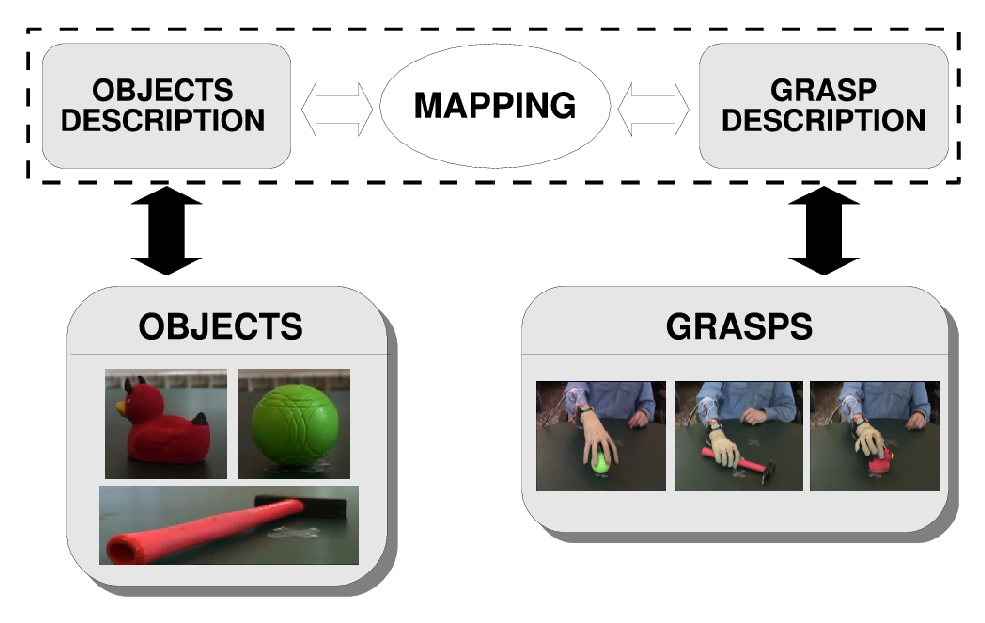
\includegraphics[width=0.7\textwidth]{images/schema_implementazione}
	\caption{An instance of the framework we propose: estimating a
     mapping between appropriate visual descriptions of objects and
     classes of grasp actions. For the time being, we assume that such
     relation is a one-to-one mapping.}
	\label{fig::implementation}
\end{figure}
%\vskip -0.5cm

In general, active modalities are not available to a biological system during the prediction phase, but only during the training phase. A paradigmatic example is that of a human infant learning how to grasp an object: by repeatedly trying to apply, e.g., a cylindric grasp to a bottle, he will learn not only to do it more and more efficiently, but also that a bottle is better be grasped cylindrically when moving it or bringing it close to the mouth. Later on, the sight of a bottle will remind the young human what one of the correct grasps is for that particular object. 
A \emph{perception-to-action map} (PAM) is the equivalent of such training for a biological system: a model to reconstruct an active modality from a passive one. The PAM of our example is a mapping from visual features of an object to motor features of the grasping action used for that object. In general such a map is many-to-many: both a hammer and a bottle can be grasped cylindrically\footnote{the nomenclature of grasp types loosely follows that of Cutkosky \cite{cutkosky}.}), and as well a mug can be handled either cylindrically or by the handle. In this work we make the simplifying assumption that for a specific object there is just one acceptable grasping action --- the PAM is one-to-one.
A PAM is useful in passive pattern recognition (e.g., classifying an object just by seeing it) since it augments the input space with PAM-reconstructed active patterns (e.g., classifying the same object from its sight \emph{and the associated grasp}). In this preliminary work we focus upon a simpler problem, namely that of checking whether, given the visual features of an object, the PAM-reconstructed grasp is (similar to) the one associated with that particular object. For example, we might train a PAM to reconstruct a pinch grip (hand posture) from the visual features of a pen; given then, in the prediciton phase, the visual features of another pen, will the PAM-reconstructed hand posture of a pinch grip look like a true pinch grip?

% We consider $5$ grasp types, shown in Figure \ref{fig::grasps}, identified by different hand postures.

% \begin{figure}
% 	\centering
% 	\includegraphics[width=0.19\textwidth]{images/cylinder}
% 	\includegraphics[width=0.19\textwidth]{images/flat}
% 	\includegraphics[width=0.19\textwidth]{images/pinch}
% 	\includegraphics[width=0.19\textwidth]{images/spherical}
% 	\includegraphics[width=0.19\textwidth]{images/tripodal}
% 	\caption{The grasp types considered in this work: \emph{(left to right)}
% 	   cylindric power grasp, flat grasp, pinch grip, spherical and
% 	   tripodal grip.}
% 	\label{fig::grasps}
% \end{figure}

In particular, what is needed is: $(i)$ a \emph{vision unit} to extract visual features from an image or a series of images, and $(ii)$ a \emph{regression unit}, which will build the PAM.
%Notice that, given our assumption that this PAM is one-to-one, a simple regression method can be used to build it, i.e., we don't have to resort to probabilistic methods such as, e.g., mixture density networks, as it has been done in literature \cite{richmond}.

%Among the various issues and possible applications taking shape from the general schema described so far, the problem we are interested to face can be stated as follows: supposing that it exists a relation between objects and actions, are we able to model it? Our idea is to exploit such relation to obtain joint information about object and action, that is predicting one of them given the other.\\
%\begin{figure}
%	\centering
%	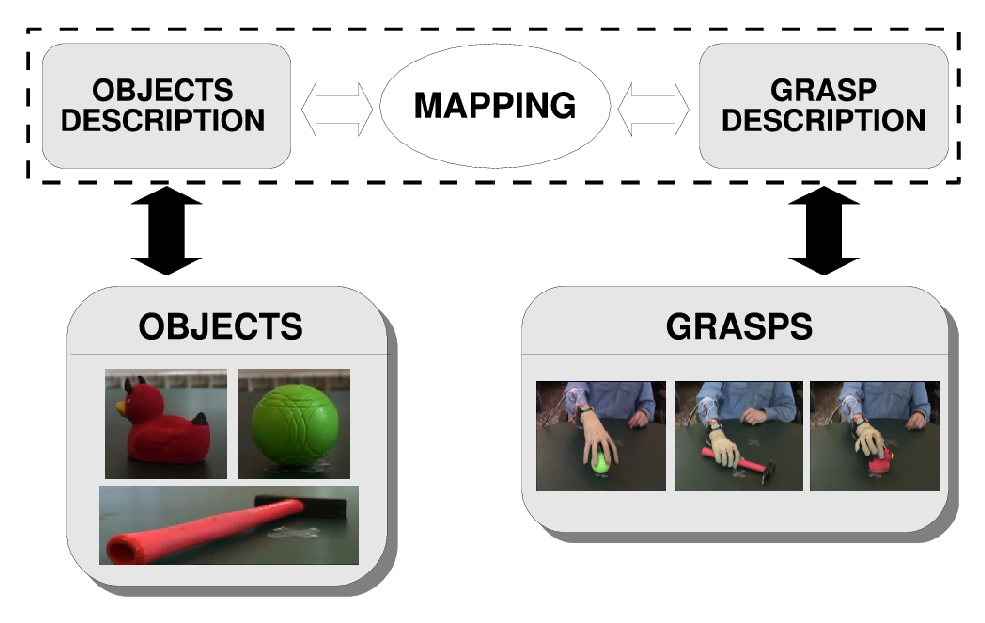
\includegraphics[width=0.7\textwidth]{images/schema_implementazione}
%	\caption{The implementation that we consider relies on estimating a mapping between appropriate descriptions of objects and classes of grasp actions. We assume that such relation is univocally determined by knowing the object.}
%	\label{fig::implementation}
%\end{figure}
%To validate this approach, we implemented a particular instance of the general schema, as shown in Fig.\ref{fig::implementation}, considering grasping actions. From the very general viewpoint we may want to consider classes of objects against classes on grasping actions. However, since our purpose here is to test the pertinence of this procedure, we start instead from the simpler hypothesis that for a specific object there is just one acceptable (class of) grasping action: in other words, we assume that the relation we are looking for can be thought of as a mono-directional mapping.\\
%\begin{figure}
%	\centering
%	\includegraphics[width=0.19\textwidth]{images/cylinder}
%	\includegraphics[width=0.19\textwidth]{images/flat}
%	\includegraphics[width=0.19\textwidth]{images/pinch}
%	\includegraphics[width=0.19\textwidth]{images/spherical}
%	\includegraphics[width=0.19\textwidth]{images/tripodal}
%	\caption{The different grasping types that we consider: from left to rigth, {\it cylinder power}, {\it flat}, {\it pinch}, {\it spherical} and {\it tripodal} grasp.}
%	\label{fig::grasps}
%\end{figure}
%We consider 5 grasp classes, as shown in Fig. \ref{fig::grasps}, ideantified by different fingers poses.
%To summarize, the framework we have in mind should include components able to:
%\begin{itemize}
%	\item model and recognize an object
%	\item extract dynamic (visual and sensorial) information related to the action
%	\item estimate a regression model to obtain information on dynamic actions starting from knowledge about objects appearance.
%\end{itemize}
%This implementation leads us to obtain a system capable of [1] modelling the relation between objects and actions in terms of mapping between appropriate descriptions to handle the multimodality, and [2] predicting the suitable grasping action for a new instance of some known object in the test phase, where motion information are not available. The latter requirement can be thought of as the capability of estimating a {\it virtual grasp}.\\
%The system accepts in input a video signal showing object and dynamic of the action, so a natural choice lies in exploiting low-level measurements extracted from images to capture their appearance. Actions can be further described by means of sensors placed on hand and fingers, allowing to capture peculiarities typical of each grasping.\\
%In the remainder of the paper we will introduce the strategy adopted to implement the system modules and present the preliminary results giving evidence of the pertinence of the proposed approach to solve the problem of interest.


\subsection{Perceptual Representations}
\label{sec:2.1}
This section describes the visual and motor features used in our framework. We begin with the visual features 
(Section \ref{sec:vis-feat}) and then continue with the motor features (Section \ref{sec:mot-feat}).

\subsubsection{Visual Features}
\label{sec:vis-feat}

% \begin{figure}
% 	\centering
% 	\includegraphics[width=0.5\textwidth]{images/objects/SchemaVisionUnit.pdf}
% 	\caption{A schematic representation of how the visual features are extracted during training(left) and test(right).}
% 	\label{fig::vision}
% \end{figure}

The visual appearance of objects is captured by a dedicated item of the framework, %(see Figure \ref{fig::vision}), 
which
can be sketched as follows.
We first select from the video sequence a set of interesting frames where the object is clearly visible. 
To avoid contamination due to background elements, 
we apply change detection by comparing the selected frames against a background model, and then
restrict our attention on the region of interest (ROI) defined by the object bounding box.
We apply to the ROI a bag-of-keypoints object description \cite{csurka-dance-2004} designed as a two steps procedure \cite{ICIAP}:

\begin{itemize}

\item  We build the global vocabulary, by putting together keypoints extracted from images of all 
the objects into the dataset. As keypoints, we consider a set of randomly sampled points whose 
patch is modeled with a vector valued  descriptor which can be seen as a fixed scale SIFT  \cite{lowe}.
K-means is adopted to cluster the descriptors: the centroids 
(or virtual features) become the words of the visual vocabulary.

\item Both training and test images are thus represented with respect to the vocabulary, with a simple 
nearest neighbor approach.  At the end, visual appearance of objects is summarized with a frequency 
histogram, whose peaks should indicate which virtual features are the most important in modelling a specific object.

\end{itemize}

Notice that the vocabulary size is a system parameter which should be tuned with respect to the complexity of 
objects, to find a trade-off between sparsity of the descriptions and capability of characterizing the objects.           

Finally a remark is in order. From the point of view of appearance-based object recognition, %from visual cues
the experimental scenario is not challenging.
We opted for such a setting in order to keep the focus of the work on the joint modelling of visual and motor inputs.
% being the focus of the work instead to give 
%evidence of the fact that motion actually improves the recognition (classification) performances.

\subsubsection{Motor Features}
\label{sec:mot-feat}
The MPR are simply the $22$ angles returned by the dataglove, considered at
the time of contact of the subject's hand with the object\footnote{A
force-sensing resistor was used to determine the instant of contact.}. The
MPR is therefore a ``snapshot'' of the subject's hand in the instant of
grasping the object.


%\begin{figure}
%	\centering
%	\includegraphics[width=0.5\textwidth]{images/schema_vision.pdf}
%	\caption{A schema of the vision unit. First, suitable frames are extracted from the sequence and objects are located by means of background subtaction (BS). SIFT descriptors of a set of random points are input of a clustering step to get to the final visual vocabulary. Finally, each image is represented with respect to the vocabulary adopting a nearest neighbour (NN) strategy (see text for details).}
%	\label{fig::vision}
%\end{figure}

%As we will discuss in Sec. \ref{sec::experiments}, the system gathers, as one input, a video sequence acting as {\it spectator}, whose focus is on object appearance. The goal of the vision unit is to process the signal to obtain a global model of a set of given objects.
%Figure \ref{fig::vision} shows the pipeline of the vision unit when considering only one object (the same procedure is applied to the whole set of objects). Among the sequence, we first select the frames showing only the object  without any occlusion, then we locate more precisely its position by means of a simple background subtraction. 
%Although in our application there is not an explicit object recognition step, it is clear from the architecture pipeline that a robust and specific object model is functional to subsequent analysis. It is worthwhile also to mention that with the terms {\it object recognition} we indicate the characterization of a specific object instance (againts the concept of categorizing classes of objects).
%We adopt an approach based on local features to describe image structures: because of their popularity a rich variety of local measurements have been proposed in the literature \cite{harris,schmid,lowe} and applied successfully to objects recognition and categorization problems (see \cite{csurka,ferrari} just to name a few). 
%Local approaches tipically include two distinct steps: keypoints extraction and description. 
%However, in our case, a keypoint based-representation often ends up into a poor description
%due to the limited size of the images. We thus built our representation by extracting enough 
%random points  guaranteeing a more homogenous sampling.
%We chose to adopt SIFT descriptors \cite{lowe,schmid2} to model image patches around these points, obtaining a set of {\it words} for each image.\\
%To avoid redundancy and include some global information in our model, we apply k-means \cite{wong}, following the well-known bag-of-words approach \cite{csurka}. 
%We thus build a {\it global} vocabulary, containing SIFT descriptions of all known objects. 
%Image representation is obtained by means of frequency histogram of visual words, selecting for each random point extracted from the image 
%the most similar visual word as nearest neighbor. A normalization step may be advisable for the subsequent data processing.

%\textbf{Questa sezione non mi e' molto chiara....ma la perceptual representation non e'
%fatta da VPR e MPR? Perche' qui descriviamo solo la vision? 
%FEATURES
%---------
%-vision: SIFT, bag of words. 50 words vocabulary, image divided in 4 parts.
%Resulting in feature vectors with 200 elements. 
%-motor: The CyberGlove returns 22 8-bit numbers linearly related to the angles 
%of the subject's hand joints. Resulting in feature vectors with 22 elements.}


\subsection{Learning the Sensor-motor Map}
\label{sec:2.2}
The VMM is supposed to be a regression strategy from visual to motor features, 
as defined above. Since the output is multivariate
(the motor features, consisting of $22$ numbers) and the input is very highly dimensional (the visual features, consisting of $200$
numbers), we decided
to enforce the VMM using neural networks. Each network was kept as
simple as possible: one hidden layer with $20$ neurons,
log-sigmoid transfer function and scaled conjugate gradient 
backpropagation. The training procedure used the early stopping
strategy, i.e. the training set was divided in a new training
and validation set. The network is evaluated on the validation set: 
when the performance stops improving, the algorithm halts. 

Most of these settings are inspired by the work of Richmond and others
\cite{papcun,richmond2007} on audio-to-motor mapping. In fact,
since each object may correspond to several grasps as it happens in reality
(recall the Section above), the relationship between the visual  and the motor features
is highly non-functional and it is in general hard, if not pointless, to
model it using a single NN. Richmond's idea was to model a \emph{probability
distribution} rather than a functional map; here we follow a somewhat more naive approach:
we define an ``archetipal grasp'' related to the specific
object observed. In the case of an object that can be grasped in only one way 
(for instance ``pig''), then the archetipal grasp will correspond 
to it. In case of an object graspable in different ways, then the 
archetipal grasp will correspond to an ``average'' grasp between those 
possible. We expect that this reconstructed grasp will have a 
positive effect on the overall performance of our object recognition system;
at the same time we hope that such representation won't get messed up
with other ones since the output space is also rather high-dimensional.


%The VMM Trying to map visual to motor information
%actually means defining a regression strategy. In our setting,
%we need a method which receive in input a SIFT feature vector
%and produces in output a sensorymotor feature vector. 
%A reasonable hypothesis is that every time we see an object 
%we are able to associate to it all the possible ways in
%which we know it can be grasped. The idea can be simplified
%supposing to define an ``archetipal grasp'',related to the specific
%object observed. In the case of an object that can be grasped in only one way 
%(for instance ``pig''), then the archetipal grasp will correspond 
%to it. In case of an object graspable in different ways, then the 
%archetipal grasp will correspond to an ``average'' grasp between those 
%possible. We expect that this reconstructed grasp will have a 
%positive effect on the overal performance of our object recognition system.
%
%We implemented this strategy using 7 neural
%networks, one for each object in the VMGdb database. All the
%neural networks are equal: 200 input values corresponding
%to the SIFT feature vector elements; 20 neurons in the hidden layer;
%22 output values corresponding to the sensorimotor feature vector 
%elemets; log-sigmoid transfer function; scaled conjugate gradient 
%backpropagation. The training procedure used the early stopping
%strategy, i.e. the training set was divided in a new training
%and validation set. The network is evaluated on the validation set: 
%when the performance stops improving, the algorithm halts. 
%
%\textbf{Solo qualche idea rozza: nella discussione finale andrebbe 
%detto che la rete neurale cosi' definita e' debole...la scelta del 
%numero nei neuroni nell'hidden layer e' 'occhiometrica': ...la teoria 
%suggerisce che dovrebbero essere di piu'...anche l'addestramento per ogni
%oggetto e' fatto usando circa 200 campioni, ma per come e' fatta la rete
%numero dei parametri che volgiamo stimare e' maggiore di 200...,
%avremmo bisogno di piu' campioni o diridurre la dimensione dei
%vettori di input ed output (sappiamo che non tutti gli elementi dei vettori
%SIFT e motor sono utili)}


\subsection{Learning the Visuo-motor Classifier}
\label{sec:2.3}
Our goal in classification is to demonstrate that the motor information is
useful in object learning and recognition. Specifically,  we want 
to show that integrating it with the visual information can 
produce a better performance, namely higher classificaton 
rate and robusteness.

To this end we consider both the visual and the motor features
labelled in terms of objects. The idea is that a classifier 
should predict which is the inspected object when the input is
 visual, motor or the combination 
of the two.
Algorithmically, this implies building a classifier over multiple cues.

In the computer vision and pattern recognition literature 
some authors have suggested different methods to combine
multiple cues. They can be all reconducted to one of the 
following three approaches: low-level, mid-level and high-level
integration \cite{Polikar2006,sanderson2004}. 
In the low-level case the features are concatenated
to define a single vector. In the mid-level approach
the different features descriptor are kept separated 
but they are integrated in a single classifier generating the
final hypothesis. The high-level method starts from
the output of different classifiers each dealing with one feature: 
the hypotheses produced are then combined together to
achieve a consensus decision.

To learn the Visuo-Motor Classifier here we decided to implement these three strategies in an SVM-based framework, and to evaluate
experimentally their suitability for the task. Specifically, 
we used the
Discriminative Accumulation Scheme (DAS, \cite{DAS}) for
the high-level, and the Multi-Cue Kernel (MCK, \cite{MCK}) for the
mid-level integration.
As already mentioned, the low-level integration consisted only in the feature concatenation, with the new vector fed to a standard SVM.


\vspace{0.5cm}

\noindent\textbf{DAS.} It is based on a weak coupling method called accumulation. Its main 
idea is that information from different cues can be summed together.

Suppose we are given $M$ object classes and for each class, a set
of $N_{j}$ training data $\{I^{j}_{i}\}_{i=1}^{N_{j}}$,
$j=1,\ldots M$. For each, we have a set of $P$ different
features so that for an object $j$ we have $P$ new training sets.
We train an SVM on every set. Kernel functions may differ from cue to
cue and model parameters can be estimated during the training step
via cross validation. Given a test image $\hat{I}$ and assuming
$M\geq2$, for each single-cue SVM we compute the distance from the
separating hyperplane $D_{j}(p)$, $p=1\ldots P$.
After collecting all the distances $\{D_{j}(p)\}_{p=1}^{P}$ for
all the $M$ objects  and the $P$ cues, we classify the image
$\hat{I}$ using the linear combination:
\begin{equation}
j^{*}=\argmax_{j=1}^{M} \left \{\sum_{p=1}^{P}a_{p}D_{j(p)} \right \}, \quad
\sum_{p=1}^{P}a_{p}=1. \label{eq:DAS}
\end{equation}
The coefficients $\{a_{p}\}_{p=1}^{P}\in \Re^{+}$ are determined
via cross validation during the training step.

\vspace{0.5cm}

\noindent\textbf{MCK.} The Multi Cue Kernel is positively
weighted linear combination of Mercer kernels, thus a Mercer kernel itself:
\begin{equation}
K_{MC}({\{T_{p}(I_{i})\}}_{p},{\{T_{p}(I)\}}_{p})=\sum_{p=1}^{P}a_{p}K_{p}(T_{p}(I_{i}),T_{p}(I)),
\; \sum_{p=1}^{P}a_{p}=1.\label{eq:MCK}
\end{equation}
In this way it is possible to perform only one classification
step, identifying the best weighting factors $a_{p}\in \Re^{+}$
through cross validation while
determining the optimal separating hyperplane. This means that the
coefficients $a_{p}$ are guaranteed to be optimal. 
 


%Here we take a mid-level approach, and we propose to use the Multi Cue Kernel
%within an SVM classifier \cite{MCK}. This method has been shown to outperform state of the art
%high- and low-level integration methods.
%
%Suppose we are given $M$ object classes and for each class, a set
%of $N_{j}$ training data $\{I^{j}_{i}\}_{i=1}^{N_{j}}$,
%$j=1,\ldots M$. For each, we have a set of $P$ different
%features so that for an object $j$ we have $P$ new training sets.
%We train an SVM on the whole set, using the Multi cue Kernel which is defined as:
%\begin{equation}
%K_{MC}({\{T_{p}(I_{i})\}}_{p},{\{T_{p}(I)\}}_{p})=\sum_{p=1}^{P}a_{p}K_{p}(T_{p}(I_{i}),T_{p}(I)),
%\; \sum_{p=1}^{P}a_{p}=1.\label{eq:MCK}
%\end{equation}
%The Multi Cue Kernel is a positively
%weighted linear combination of Mercer kernels, thus a Mercer kernel itself.
%By using this mid-level integration strategy, 
%it is possible to perform only one classification
%step, identifying the best weighting factors $a_{p}\in \Re^{+}$
%through cross validation while
%determining the optimal separating hyperplane. This means that the
%coefficients $a_{p}$ are guaranteed to be optimal.
%
%To assess our results, we implemented also a low-level and a high-level, SVM-based approaches.
%For the low-level case, we simply concatenated the features to form a single vector, and fed it as input to an SVM. 
%For the high-level case, we chose the Discriminative Accumulation Scheme (DAS, \cite{DAS}) that showed very high 
%performances on several object
%recognition and robot vision applications \cite{DAS, pronobis_etal_icra2008}.
%
%




\subsection{Motor Grasp Priming}
\label{sec:2.4}
\input{grasp-priming}

\subsection{Visuo-motor Object Recognition}
\label{sec:2.5}
\input{vm-obj}

\section{Experiments}
\label{exper}
\input{hat-exper}

\subsection{The Database}
\label{sec:3.1}
\begin{figure*}[tb]
	\centering
	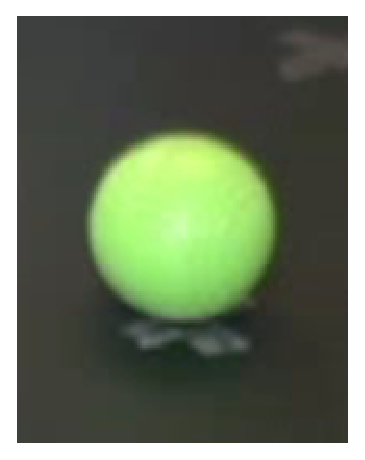
\includegraphics[height=1.75cm]{images/objects/palla}
	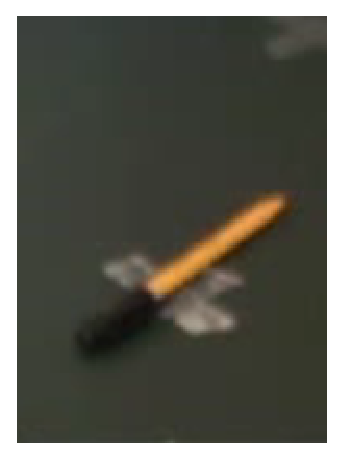
\includegraphics[height=1.75cm]{images/objects/penna}
	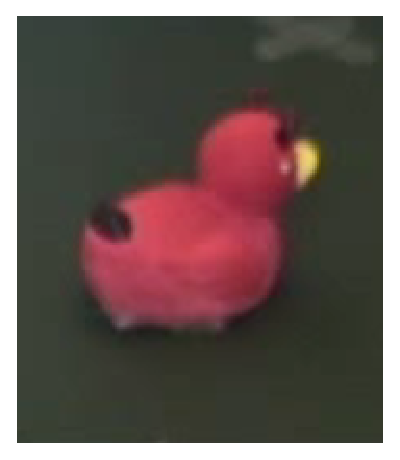
\includegraphics[height=1.75cm]{images/objects/papera}
	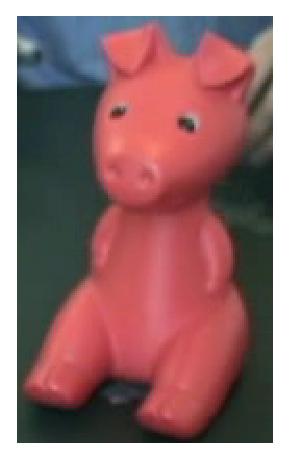
\includegraphics[height=1.75cm]{images/objects/porcellino}
	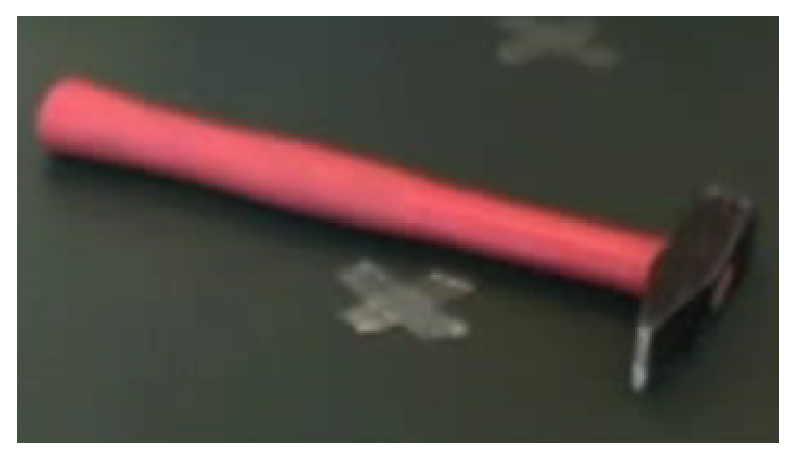
\includegraphics[height=1.75cm]{images/objects/martello}
	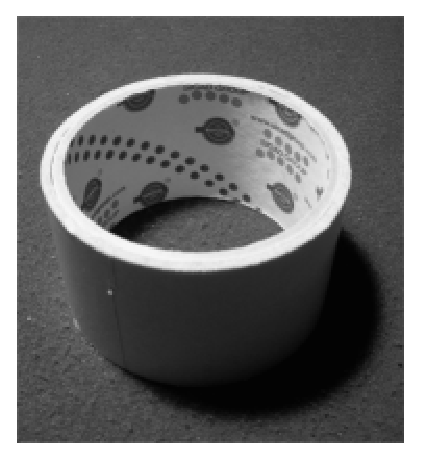
\includegraphics[height=1.75cm]{images/objects/scotch}
	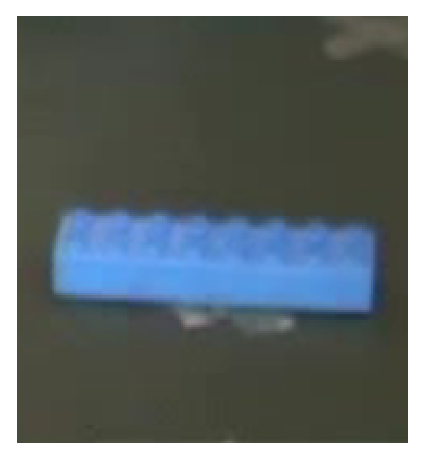
\includegraphics[height=1.75cm]{images/objects/lego}\\
	\vskip 0.1cm
	\includegraphics[width=0.12\textwidth]{images/objects/cylinder}
	\includegraphics[width=0.12\textwidth]{images/objects/flat}
	\includegraphics[width=0.12\textwidth]{images/objects/pinch}
	\includegraphics[width=0.12\textwidth]{images/objects/spherical}
	\includegraphics[width=0.12\textwidth]{images/objects/tripodal}
	\caption{Top row: the objects used in our experiments. Bottom, the grasp types we consider: \emph{(left to right)} cylindric power grasp, flat grasp, pinch grip, spherical and
	tripodal grip.}
	\label{fig::grasps}
\end{figure*}

The VMGdB dataset is built considering 7 different objects ((see Fig. \ref{fig::grasps}), top) and 5 grasps ((see Fig. \ref{fig::grasps}), bottom).
 20 different actors participated to the acquisition, during which  
 each object was grasped in one or more  ways, according to the many-to-many relationship reported in Table \ref{tab:manytomany}. In total
we consider 13 different pairs (grasp,object), and, for each triple {\em (object, grasp, actor)}, we acquired 20 replicates of the grasping experiment.
 
 {\small
\begin{table}
\begin{tabular}{c | c c c c c c c}
& ball & pen & duck & pig & hammer & tape & lego brick \\
\hline \\
cylindr. pow. & & & & X & & & \\
flat & & & &  & X & & X \\
pinch & & X & X & & & X & X \\
spherical & X & & & & & X & \\
tripodal & X & X & X & & & X & 
\end{tabular}
\caption{\label{tab:manytomany} Mapping grasps-objects. Each actor performs grasping actions on 13
object-grasp type pairs.}
\end{table}
}
 
We obtained 5200 experiments {\em (object, grasp, actor, expnum)}, and for each of them the VMGdB stores the following information:
\begin{itemize}
\item {\bf Visual information.} 2 video sequences  acquired by 2 color cameras with different focus -- one is the object, the other one is the grasping action. The video sequences
are associated to 2 data files reporting the video frames time-stamps, allowing for synchronization with the sensor data;
\item {\bf Hand posture sensor information.} 1 data file containing the hand posture sensor data acquired by a CyberGlove
\cite{cyberglove}. 
For each posture the glove returns $22$ $8$-bit numbers linearly related to the angles of the actor's hand joints. 
The sensors describe the position of the three phalanxes of each finger (for the thumb, rotation and two phalanxes), the four finger-to-finger
abductions, the palm arch, the wrist pitch and the wrist yaw. Again, the sensor data are associated to acquisition time-stamps for synchronization. 
\end{itemize}



\subsection{Results for the Motor Grap Priming}
\label{sec:3.2}
FIXME NICOLETTA, ANNALISA, LUCA, FRANCESCA


\subsection{Results for Visuo-motor Object Recognition}
\label{sec:3.3}
\input{vm-obj-results}

\section{Conclusions}
This paper presented a theoretical framework for joint modelling of visual and motor data for multimodal object recognition.
The key feature of our approach is the learning of a Visuo-Motor Map between the two modalities during training.
The existence of this map makes it possible to benefit from the multimodal nature of the model even when the motor data
is not perceived by the system. Experiments confirm the validity of our approach, showing a gain in performance
of up to 7.6\% and 2.4\% when using both modalities, compared to results achieved using vision only.

%In this paper we have shown that even a simple approach to sensorimotor learning
%can significantly improve the performance of a traditional classifer. The performance
%of our VMM-enhanced object classification system is such that .... \textbf{numeri dagli
%esperimenti}. The VMM has been obtained so far in the most straightforward way, that
%is, by applying a standard neural network to visual features of objects, and having
%it map onto motor features of an associated grasp.

The data upon which our experiments have been carried on are collected in the
CONTACT Visuo-Motor Grasping dataBase (VMGdB), which we envision as a testbed and
a benchmark for all researchers interested in investigating the nature of (human and
robotic) grasping, and its ties to object recognition. %In fact, in this work we have
%neglected a lot of potentially useful information contained in the database, for instance
%the dynamics associated with the reaching phase, prior to grasping, which is well-known
%to carry substantial information about it \cite{174427,santello}.

\noindent
{\bf Future Work.} The current implementation of the framework contains several simplifying assumptions, each corresponding to 
ongoing and future research directions:
\begin{enumerate}
\item {\em Dynamic of the data.}
In this work we have
neglected a lot of potentially useful information coming from the dynamics associated with the reaching phase, prior to grasping.
This is well-known
to carry substantial information about it \cite{174427,santello}. We plan to include the dynamic in the representation of motor and 
also visual features: indeed the dynamic changes in the object state associated with its manipulation are an important cue on the
object's identity \cite{gupta_davis_cvpr2008,kjellstrom_etal_eccv2008}. This research direction will likely lead us to move
from grasping postures to grasping actions, and therefore affordance-based object representations.

\item {\em Shape-based visual representations.}
While here we used an appearance-based visual representation for the object, we are fully aware that this visual information
is weakly correlated with the grasping and therefore makes the life of the mapping function much harder. We plan in the future to
represent objects based on shape information. This will lead to visual information complementary to the grasp hand posture (the
configuration of the hand at the moment of the grasp can be seen as a motor-based information regarding the shape of the object).
We also expect that a shape-based visual representation will make it possible to build categorical object models based on their
shape, i.e. graspability. This might lead to better defined VMMs, and it would greatly help in the case of large number
objects. 


\item {\em Learning of the Visuo-Motor Map.}
Experimental results  indicate that the ``real'' motor features, that is, the
grasping hand postures as recorded by the data glove, contain much more information
than the visual features alone. Therefore, if one were able to extract more (or better)
motor information from the sight of an object, that is, to build a better VMM,
the situation could improve further. One immediate direction for this line of research
is that of abandoning the somewhat artificial notion of an archetypal grasp associated
with an object, and start training a VMM in order for it to reconstruct a
\emph{probability distribution} over grasps. This would correspond to enhancing an
object model with a possible set of grasps, rather than with one grasp only; a
further, important step toward the re-definition of an object in terms of its
affordances.
We are currently studying an extended version of the VMM architecture based on vector-valued regression to explicitly take into account the many-to-many relationship between objects and grasps. In this case, instead of learning the map between an object and an average grasp, we would learn the map between an object and a vector of the possible grasps. At run time this would allow us to associate the most probable grasp to the object under consideration.


\end{enumerate}


\begin{thebibliography}{4}

\bibitem{rizz} Rizzolatti, G., Craighero, L.: The Mirror-Neuron System. Annual Review of Neuroscience. 27:169-92 (2004)

\bibitem{harris} Harris, C., Stephens, M.: A Combined Corner and Edge Detector. Proceedings of The Fourth Alvey Vision Conference. pp. 147-151 (1988)

\bibitem{schmid} Mikolajczyk, K., Schmid, C.:Scale and Affine Invariant Interest Point Detectors. In IJC. V 60(1):63-86 (2004)

\bibitem{lowe} Lowe, D. G.: Distinctive Image Features from Scale-Invariant Keypoints. International Journal of Computer Vision. 60 (2): 91–110 (2004) 

%\bibitem{lindeberg} Lindeberg, T.: Feature Detection with Automatic Scale Selection. International Journal of Computer Vision. 30 (2): 79–116 (1998)

%\bibitem{perona} Moreels, P., Perona, P.: Evaluation of Features Detectors and Descriptors Based on 3D Objects. In ICCV. (2005)

\bibitem{schmid2} Mikolajczyk, K., Schmid, C.:A Performance Evaluation of Local Descriptors. Trans on PAMI. 27(10) (2005)

%\bibitem{leibe} Leibe, B., Mikolajczyk, K., Schiele, B.: Efficient Clustering and Matching for Object Class Recognition. In BMVC. (2006)

\bibitem{csurka} Csurka, G., Dance, C.R., Fan, L., Bray, C.: Visual Categorization with Bag of Keypoints. In ECCV. (2004)

\bibitem{ferrari} Ferrari, V., Tuytelaars, T., Van Gool, L.: Simultaneous Object Recognition and Segmentation from Single or Multiple Model Views. IJVC. 67(2) (2006)

\bibitem{LoGerfo08Spectral} Lo Gerfo, L., Rosasco, L., Odone, F., De Vito, E., Verri, A.:
  Spectral Algorithms for Supervised Learning. Neural Computation. 20(7) (2008)

 \bibitem{Yao07Early}
   Yao, Y., Rosasco, L., Caponnetto, A.: On Early Stopping in Gradient Descent Learning.
   Constructive Approximation. 26(2) (2007)

\bibitem{MicchPon05Onlearning} Micchelli, C.~A., Pontil, M.: On learning vector-valued functions.
  Neural Computation. 17 (2005)

\bibitem{dev04representer} De Vito, E., Rosasco, L., Caponnetto, A., Piana, M.,	Verri, A.:Some Properties of Regularized Kernel Methods. Journal of Machine Learning Research. 5 (2004)

\bibitem{preprint} Baldassarre, L., Barla, A.,  Rosasco, L., Verri, A.:
Learning vector valued functions with spectral regularization. (preprint)

% \bibitem{jung} Hye-Won, J., Yong-Ho, S., Ryoo, M.S., Yang, H.S: Affective Communication System with Multimodality for a Humanoid Robot, AMI.
% 4th IEEE/RAS International Conference on Humanoid Robots. 2 (2004)

% \bibitem{kruger} Kr$\ddot{u}$ger, N., Felsberg, M., W$\ddot{o}$rg$\ddot{o}$tter, F.: Processing Multi-modal Primitives from Image Sequences. 4th ICSE Symposium on Engineering of Intelligent Systems. (2004) 

% \bibitem{yang} Yang, G., Lin, Y., Bhattacharya, P.: Multimodality Inferring of Human Cognitive States Based on Integration of Neuro-Fuzzy Network and Information Fusion Techniques. EURASIP Journal on Advances in Signal Processing. 8(2008)

\bibitem{gallese} Gallese, V., Fadiga, L., Fogassi, L., Rizzolatti, G.: Action Recognition in the Premotor Cortex. Brain. 119, 593–609 (1996)

% \bibitem{grans} Granström, B. House, D., Karlsson, I.: Multimodality in Language and Speech Systems. Text, Speech and Language Technology. 19(2002)

\bibitem{metta} Metta, G., Sandini, G., Natale, L., Craighero, L., Fadiga, L.: Understanding  Mirror Neurons: A Bio-Robotic Approach. Interaction Studies. 7, 197–232, (2006)

% \bibitem{caputo} Luo, J., Pronobis, A., Caputo, B.: SVM-based Transfer of Visual Knowledge Across Robotic Platforms. 5th International Conference on Computer Vision Systems. (2007)

% \bibitem{thrun} Thrun, S., Mitchell, T.: Lifelong Robot Learning. Robotics and Autonomoues Systems. 15 (1995)

% \bibitem{malak} Malak, R.J., Khosla, P.K.: A Framework for the Adaptive Trasfer of Robot Skill Knowledge Using Reinforcement Laerning Agents. Proc of ICRA. (2001)

% \bibitem{barto} Konidaris, G., Barto, A.G.: Autonomous Shaping: Knowledge Transfer in Reinforcement Learning. Proc. of ICML. (2006) 

\bibitem{wong} Hartigan, J. A., Wong, M. A.: A K-Means Clustering Algorithm". Applied Statistics. 28(1) (1979) 

\bibitem{cutkosky} Cutkosky, M.: On grasp choice, grasp models and the design of hands for manufacturing tasks. IEEE Transactions on Robotics and
Automation. (1989)

\bibitem{2007.AR} Castellini, C., Orabona, F., Metta, G., Sandini, G.: Internal Models of Reaching and Grasping. Advanced Robotics. 21(13) (2007)

%\bibitem{papcun} Papcun, G., Hochberg, J., Thomas, T. R., Laroche, F., Zacks, J., Levy, S.: Inferring articulation and recognizing gestures from acoustics with a neural network trained on x-ray microbeam data. J Acoust Soc Am. 92(2) (1992)

%\bibitem{richmond} Richmond, K., King, S., Taylor, P.: Modelling the uncertainty in recovering articulation from acoustics. Computer Speech and Language. 17 (2003)

\bibitem{bulmann02boosting} Buhlmann, P.: Boosting for High-Dimensional Linear Models". Annals of Statistics. 34(2), 559–58 (2006)

\bibitem{micchelli04kernels} Micchelli, C. A., Pontil, M.: Kernels for Multi-task Learning. NIPS (2004)

\bibitem{rifkin03rlsc} Rifkin, R., Yeo, G., Poggio, T.: Regularized Least-Squares Classification. Advances in Learning Theory: Methods, Models and Applications. (2003) 

\bibitem{pontil08transferlearning} Argyriou, A., Maurer, A., Pontil, M.: An Algorithm for Transfer Learning in a Heterogeneous Environment. ECML/PKDD. (1) 71-85 (2008) 

\bibitem{jacob08clusteredmtl} Jacob, L., Bach, F., Vert, J.P.: Clustered Multi-Task Learning: a Convex Formulation. NIPS. (2008) 

\end{thebibliography}
\end{document}
